\section{RNN Architectures}
\begin{frame}{}
  \LARGE RNN : \textbf{Architecture}
\end{frame}

\begin{frame}{RNN Architecture: Unrolled View}
  \begin{columns}[c]
    \begin{column}{0.52\textwidth}
      \textbf{Unrolled RNN:} \\
      An RNN is essentially a chain of repeating neural network modules, one for each time step.
      \vspace{0.5em}

      \textbf{Each time step shares the same parameters:}
      \begin{itemize}
        \item[\textcolor{red}{$\blacktriangleright$}] Input $x_t$
        \item[\textcolor{red}{$\blacktriangleright$}] Hidden state $h_t$
        \item[\textcolor{red}{$\blacktriangleright$}] Output $y_t$
      \end{itemize}

      \textcolor{blue}{\textbf{Key Idea}} \\
      Temporal representation without increasing parameter count!
    \end{column}
    \begin{column}{0.48\textwidth}
      \centering
      \begin{figure}
        \centering
        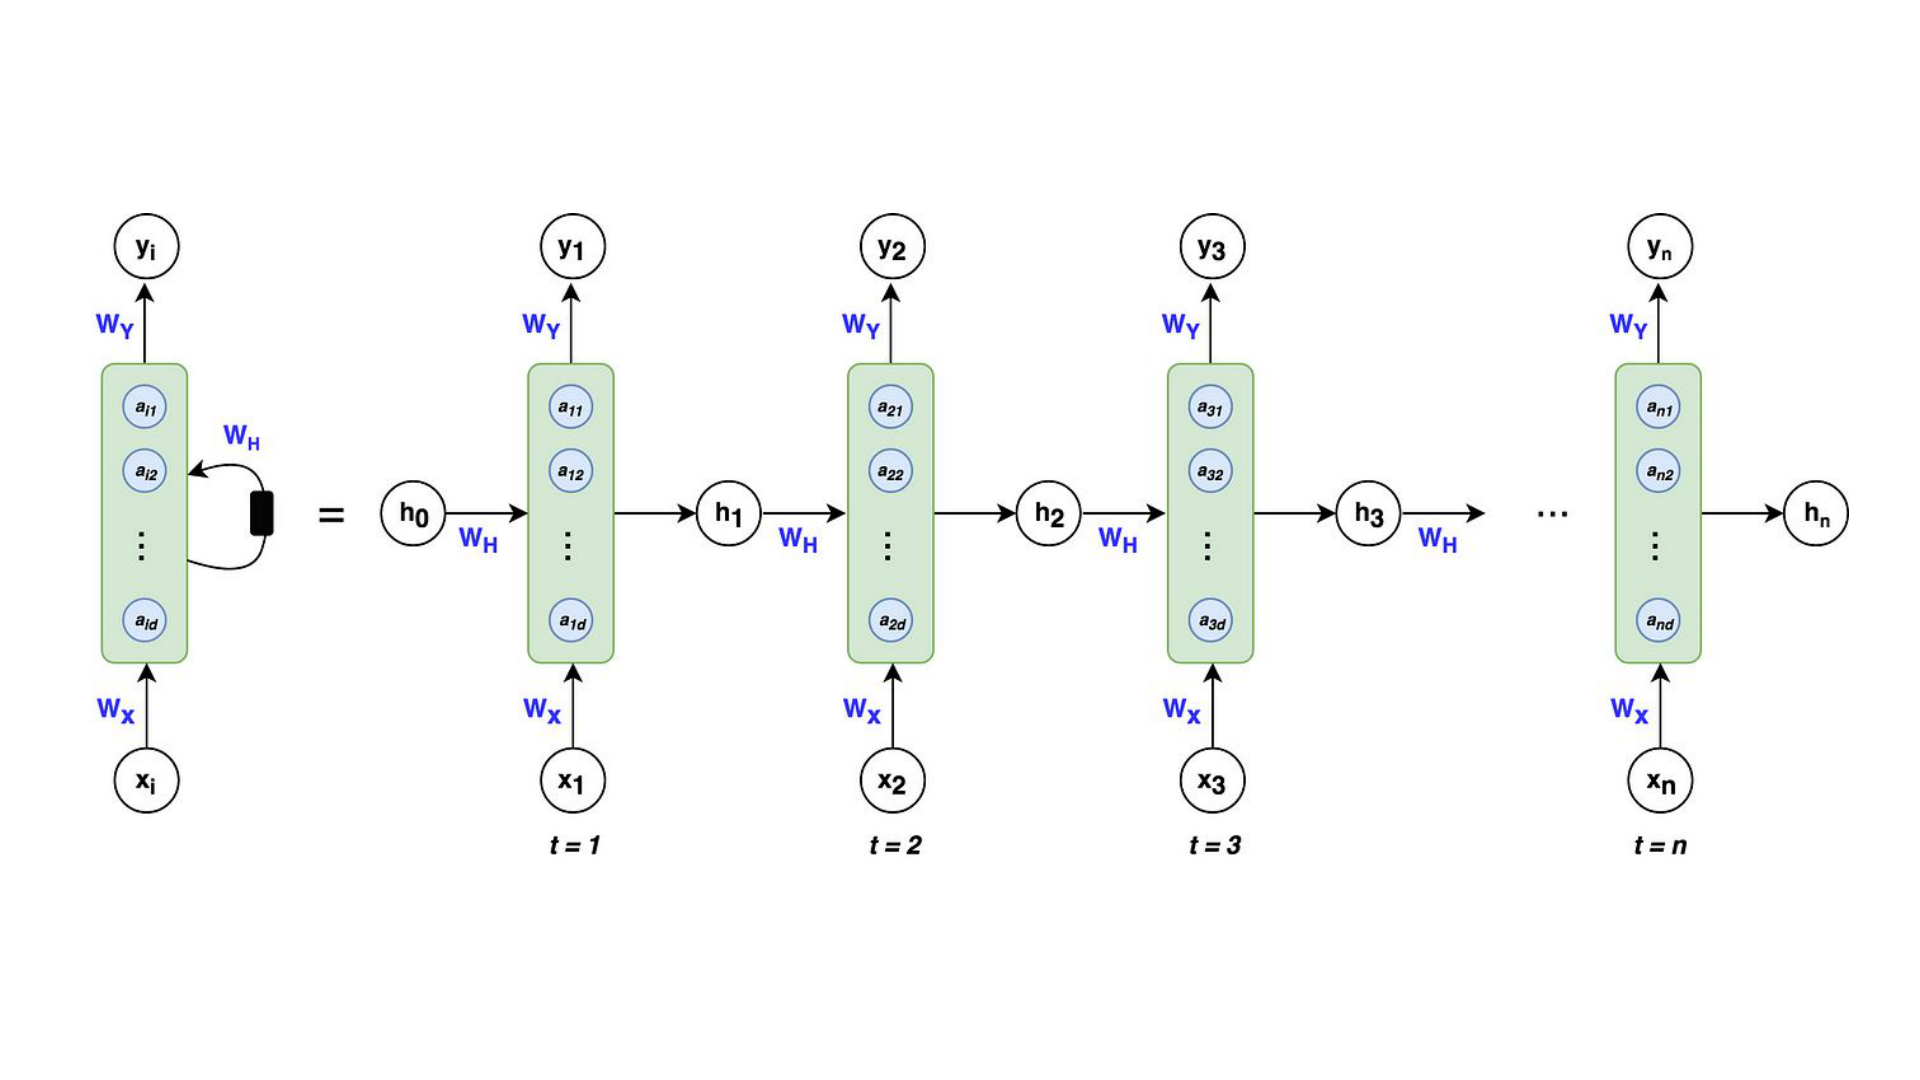
\includegraphics[width=0.99\linewidth,keepaspectratio]{images/rnn-lstm-gru/rnn_unrolled_computation_graph_full.png}
        \caption*{\tiny Source: B. Khuong, ``The Basics of Recurrent Neural Networks (RNNs),'' Towards AI, 2019}
      \end{figure}
    \end{column}
  \end{columns}
\end{frame}

\begin{frame}{Vanilla Neural Network}
  \begin{figure}
    \centering
    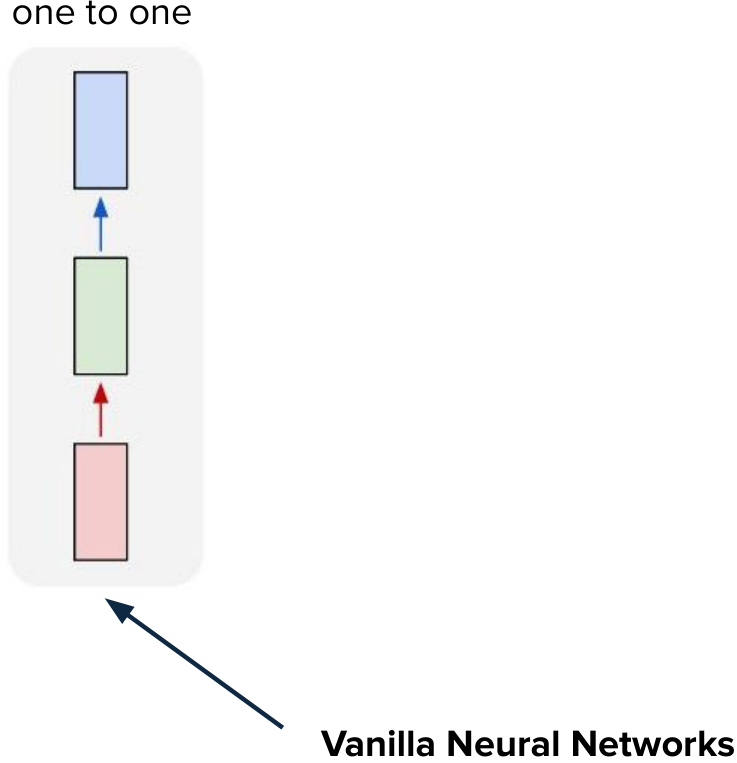
\includegraphics[width=0.9\paperwidth,height=0.66\paperheight,keepaspectratio]{images/rnn-lstm-gru/rnn_one_to_one_vanilla.png}
    \caption*{\tiny Source: Stanford CS231n (2022), Lecture 10: Recurrent Neural Networks; figure after A. Karpathy, ``The Unreasonable Effectiveness of Recurrent Neural Networks'' (2015)}
  \end{figure}
\end{frame}

\begin{frame}{One to One}
  \begin{figure}
    \centering
    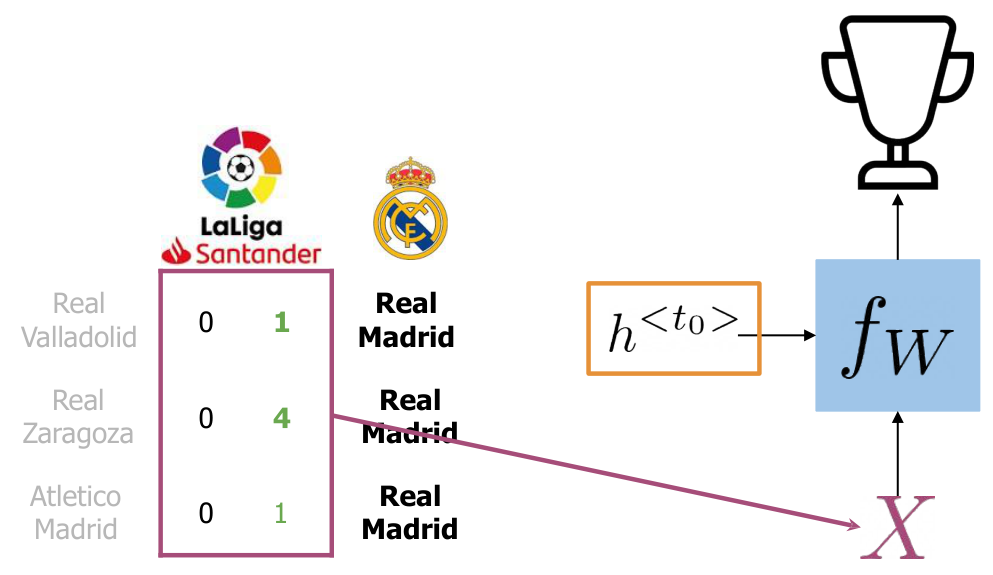
\includegraphics[width=0.8\paperwidth,height=0.66\paperheight,keepaspectratio]{images/rnn-lstm-gru/rnn_laliga_real_madrid_example.png}
    \caption*{\tiny Source: DeepLearning.AI NLP Specialization, Course 3: Natural Language Processing with Sequence Models, Week 2 (Y. Bensouda Mourri \& L. Kaiser)}
  \end{figure}
\end{frame}

\begin{frame}{RNN: Process Sequences}
  \begin{figure}
    \centering
    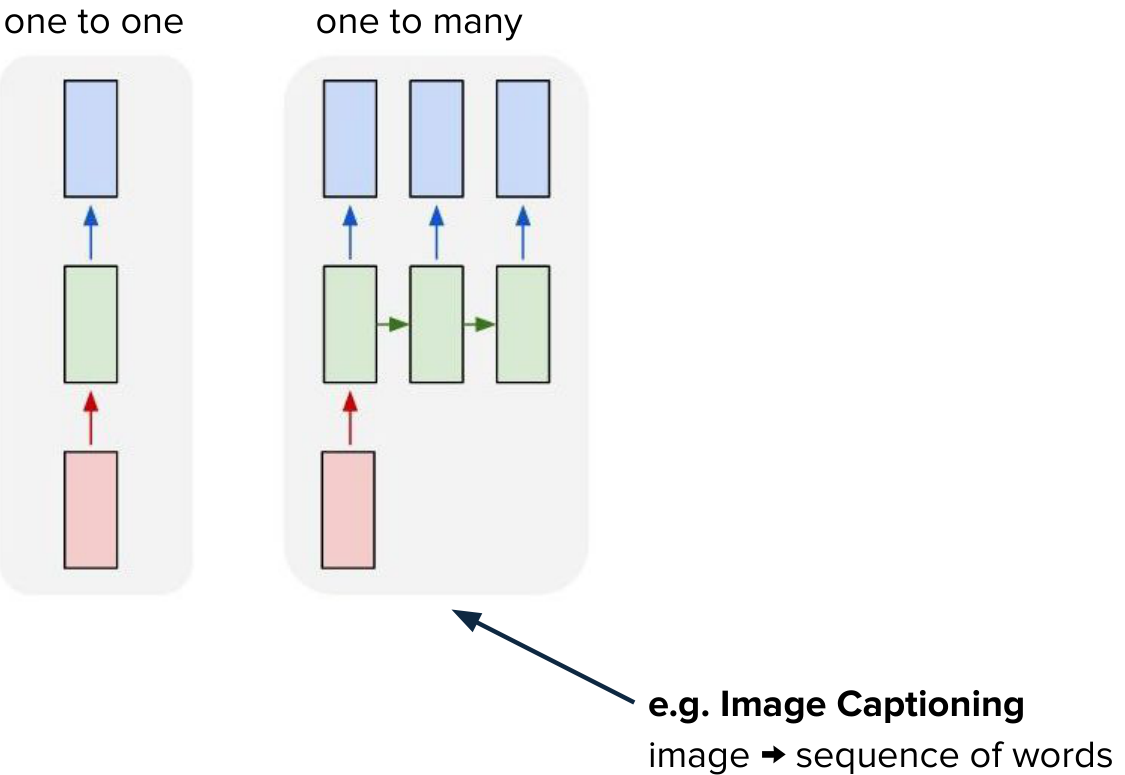
\includegraphics[width=0.8\paperwidth,height=0.66\paperheight,keepaspectratio]{images/rnn-lstm-gru/rnn_one_to_many_image_captioning.png}
    \caption*{\tiny Source: Stanford CS231n (2022), Lecture 10: Recurrent Neural Networks; figure after A. Karpathy, ``The Unreasonable Effectiveness of Recurrent Neural Networks'' (2015)}
  \end{figure}
\end{frame}

\begin{frame}{One to Many}
  \begin{figure}
    \centering
    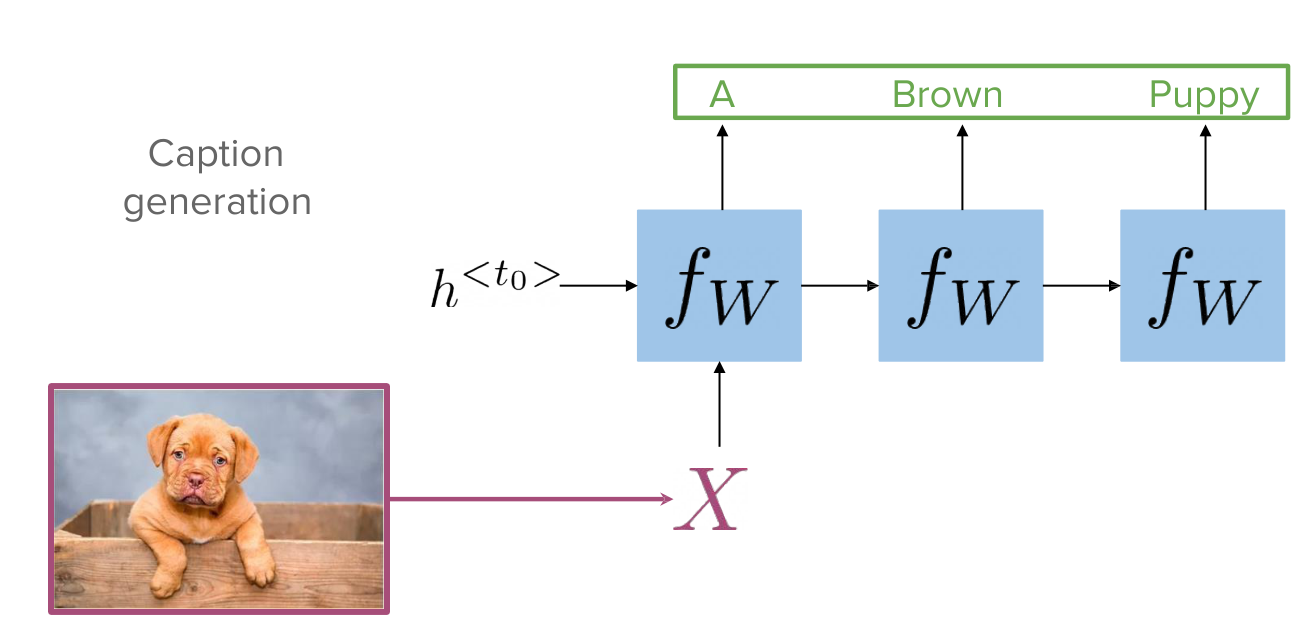
\includegraphics[width=0.9\paperwidth,height=0.66\paperheight,keepaspectratio]{images/rnn-lstm-gru/rnn_caption_generation_brown_puppy.png}
    \caption*{\tiny Source: DeepLearning.AI NLP Specialization, Course 3: Natural Language Processing with Sequence Models, Week 2 (Y. Bensouda Mourri \& L. Kaiser)}
  \end{figure}
\end{frame}

\begin{frame}{RNN: Process Sequences}
  \begin{figure}
    \centering
    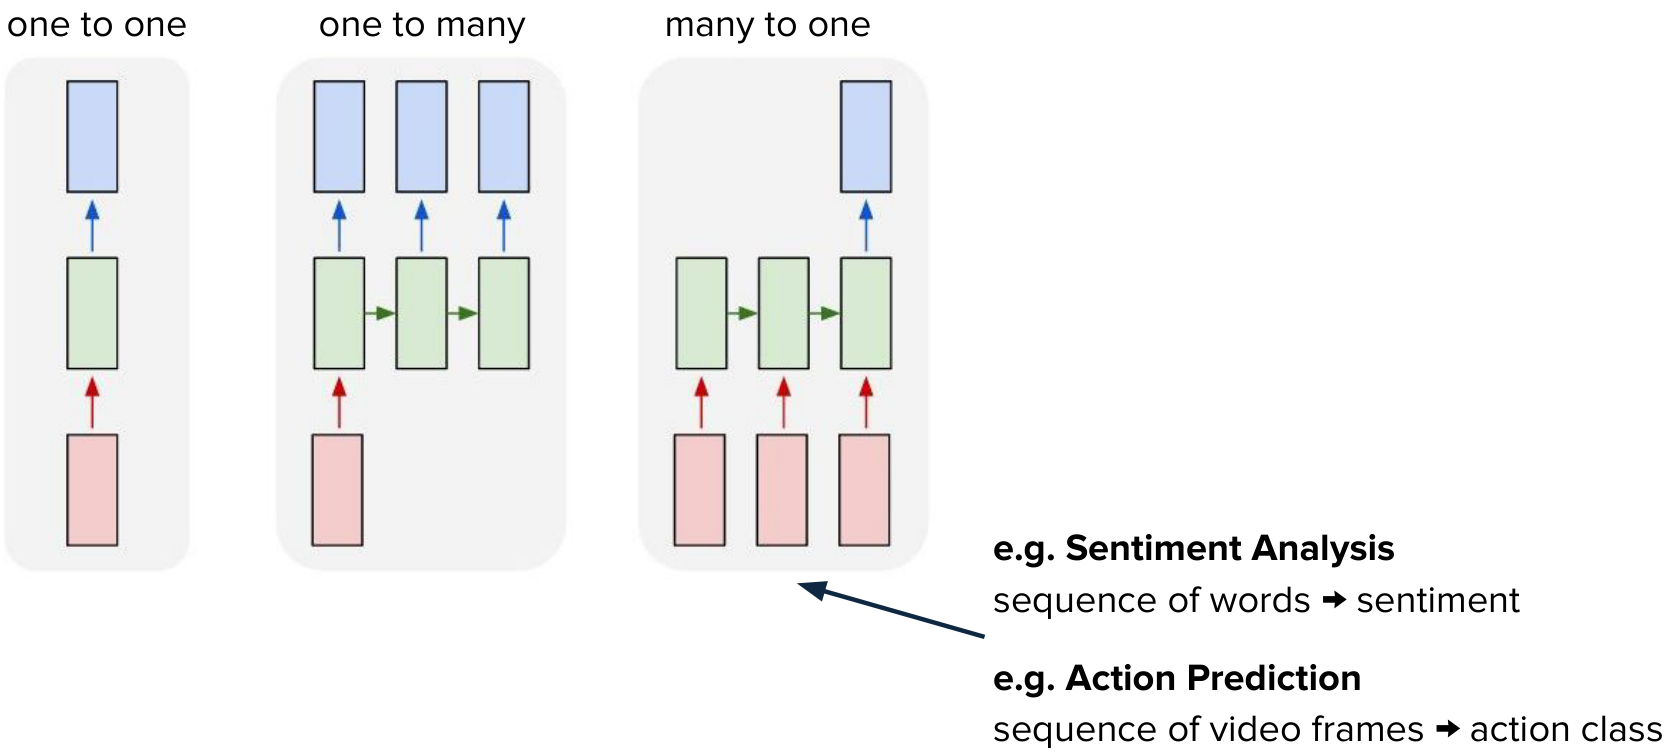
\includegraphics[width=0.9\paperwidth,height=0.66\paperheight,keepaspectratio]{images/rnn-lstm-gru/rnn_many_to_one_sentiment.png}
    \caption*{\tiny Source: Stanford CS231n (2022), Lecture 10: Recurrent Neural Networks; figure after A. Karpathy, ``The Unreasonable Effectiveness of Recurrent Neural Networks'' (2015)}
  \end{figure}
\end{frame}

\begin{frame}{Many to One}
  \begin{figure}
    \centering
    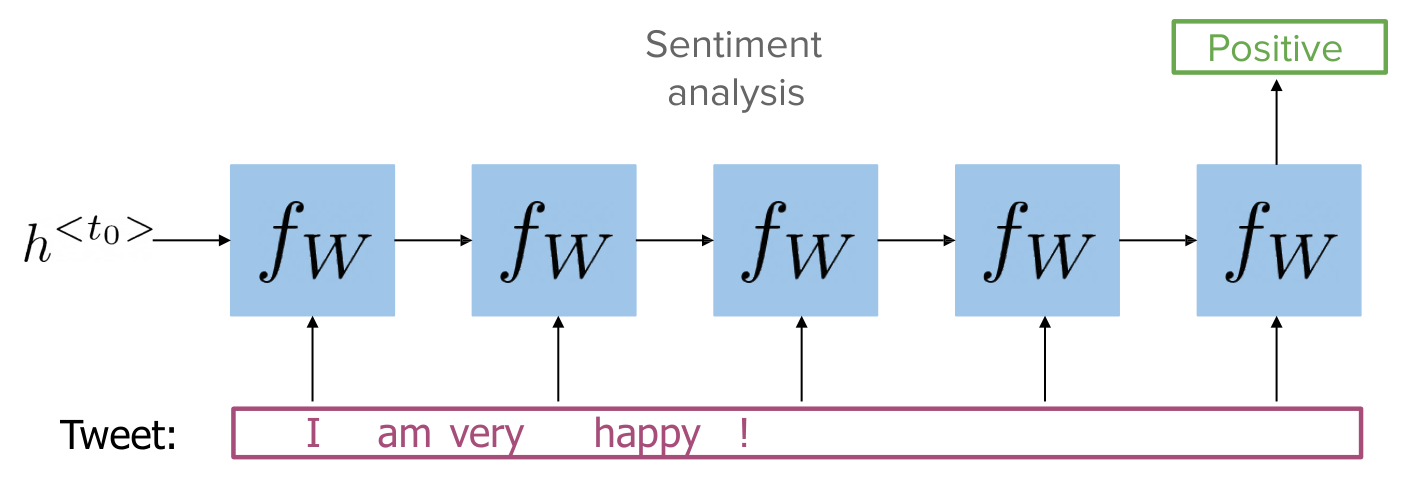
\includegraphics[width=\linewidth,height=0.66\paperheight,keepaspectratio]{images/rnn-lstm-gru/rnn_sentiment_analysis_tweet.png}
    \caption*{\tiny Source: DeepLearning.AI NLP Specialization, Course 3: Natural Language Processing with Sequence Models, Week 2 (Y. Bensouda Mourri \& L. Kaiser)}
  \end{figure}
\end{frame}

\begin{frame}{RNN: Process Sequences}
  \begin{figure}
    \centering
    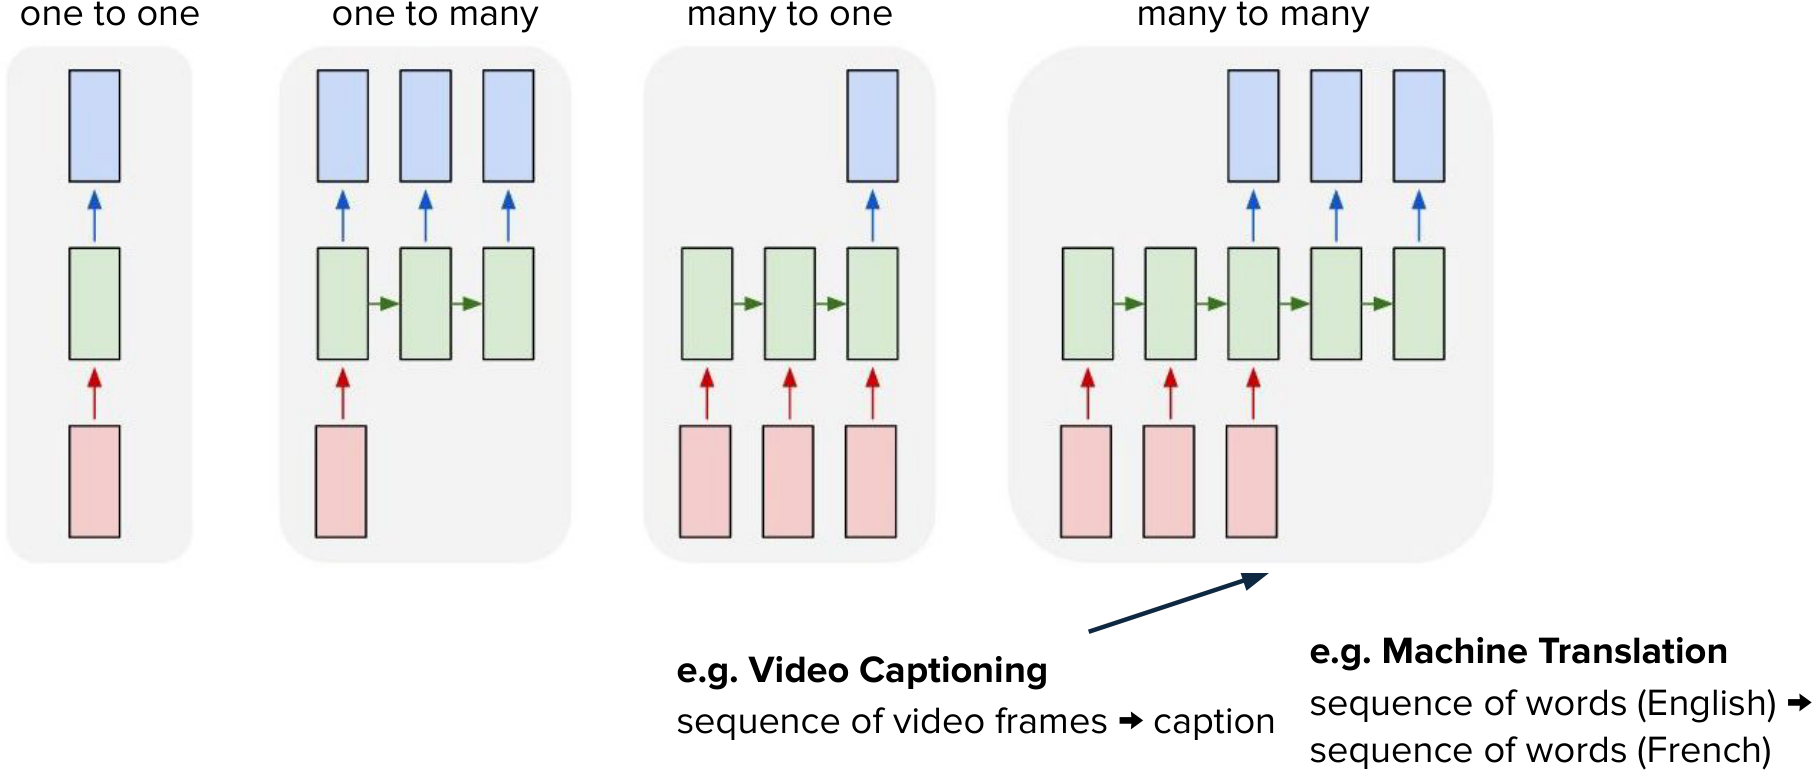
\includegraphics[width=0.9\paperwidth,height=0.66\paperheight,keepaspectratio]{images/rnn-lstm-gru/rnn_many_to_many_machine_translation.png}
    \caption*{\tiny Source: Stanford CS231n (2022), Lecture 10: Recurrent Neural Networks; figure after A. Karpathy, ``The Unreasonable Effectiveness of Recurrent Neural Networks'' (2015)}
  \end{figure}
\end{frame}

\begin{frame}{Many to Many}
  \begin{figure}
    \centering
    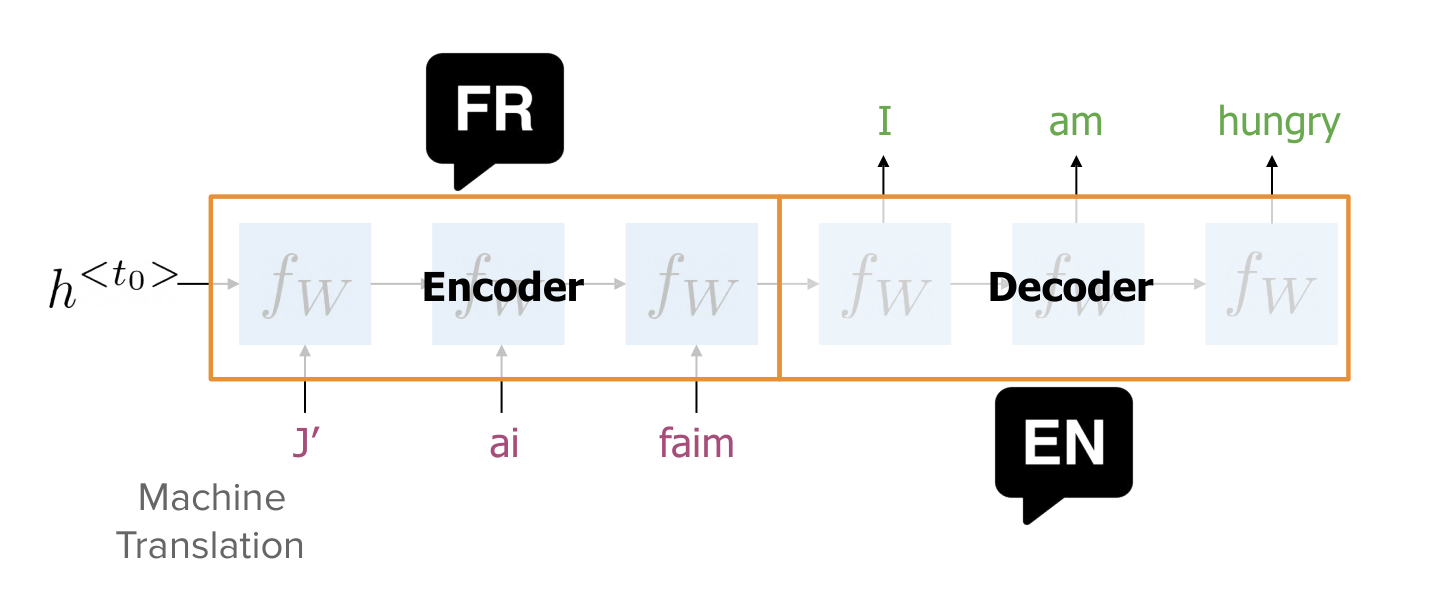
\includegraphics[width=\linewidth,height=0.66\paperheight,keepaspectratio]{images/rnn-lstm-gru/rnn_encoder_decoder_translation.png}
    \caption*{\tiny Source: DeepLearning.AI NLP Specialization, Course 3: Natural Language Processing with Sequence Models, Week 2 (Y. Bensouda Mourri \& L. Kaiser)}
  \end{figure}
\end{frame}

\begin{frame}{RNN: Process Sequences}
  \begin{figure}
    \centering
    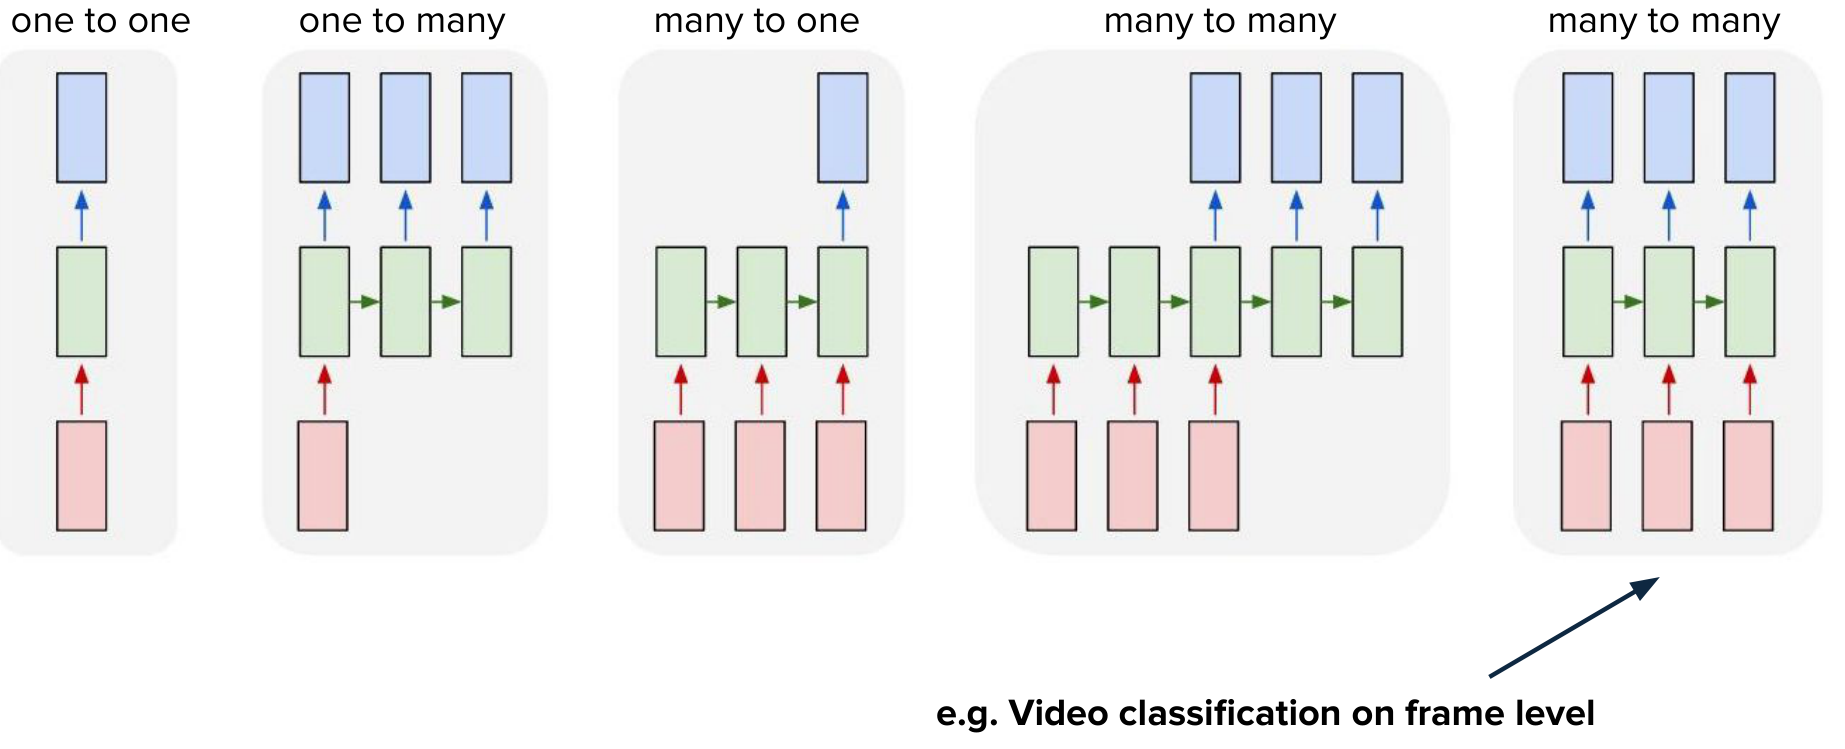
\includegraphics[width=\linewidth,height=0.66\paperheight,keepaspectratio]{images/rnn-lstm-gru/rnn_many_to_many_video_classification.png}
    \caption*{\tiny Source: Stanford CS231n (2022), Lecture 10: Recurrent Neural Networks; figure after A. Karpathy, ``The Unreasonable Effectiveness of Recurrent Neural Networks'' (2015)}
  \end{figure}
\end{frame}

\begin{frame}{Recurrent Neural Network}
  \begin{figure}
    \centering
    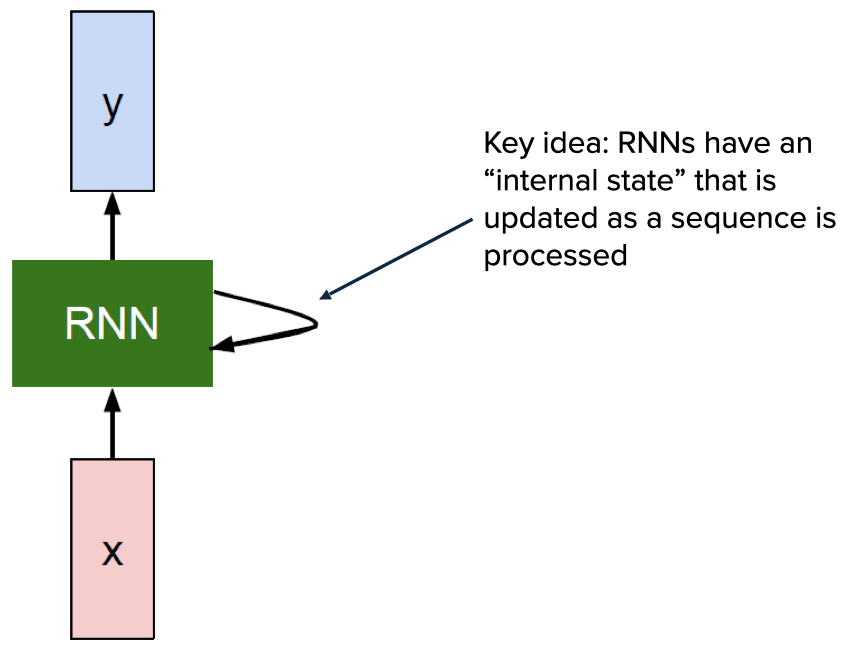
\includegraphics[width=0.9\paperwidth,height=0.66\paperheight,keepaspectratio]{images/rnn-lstm-gru/rnn_internal_state_key_idea.png}
    \caption*{\tiny Source: Stanford CS231n (2022), Lecture 10: Recurrent Neural Networks}
  \end{figure}
\end{frame}

\begin{frame}{Unrolled RNN}
  \centering
  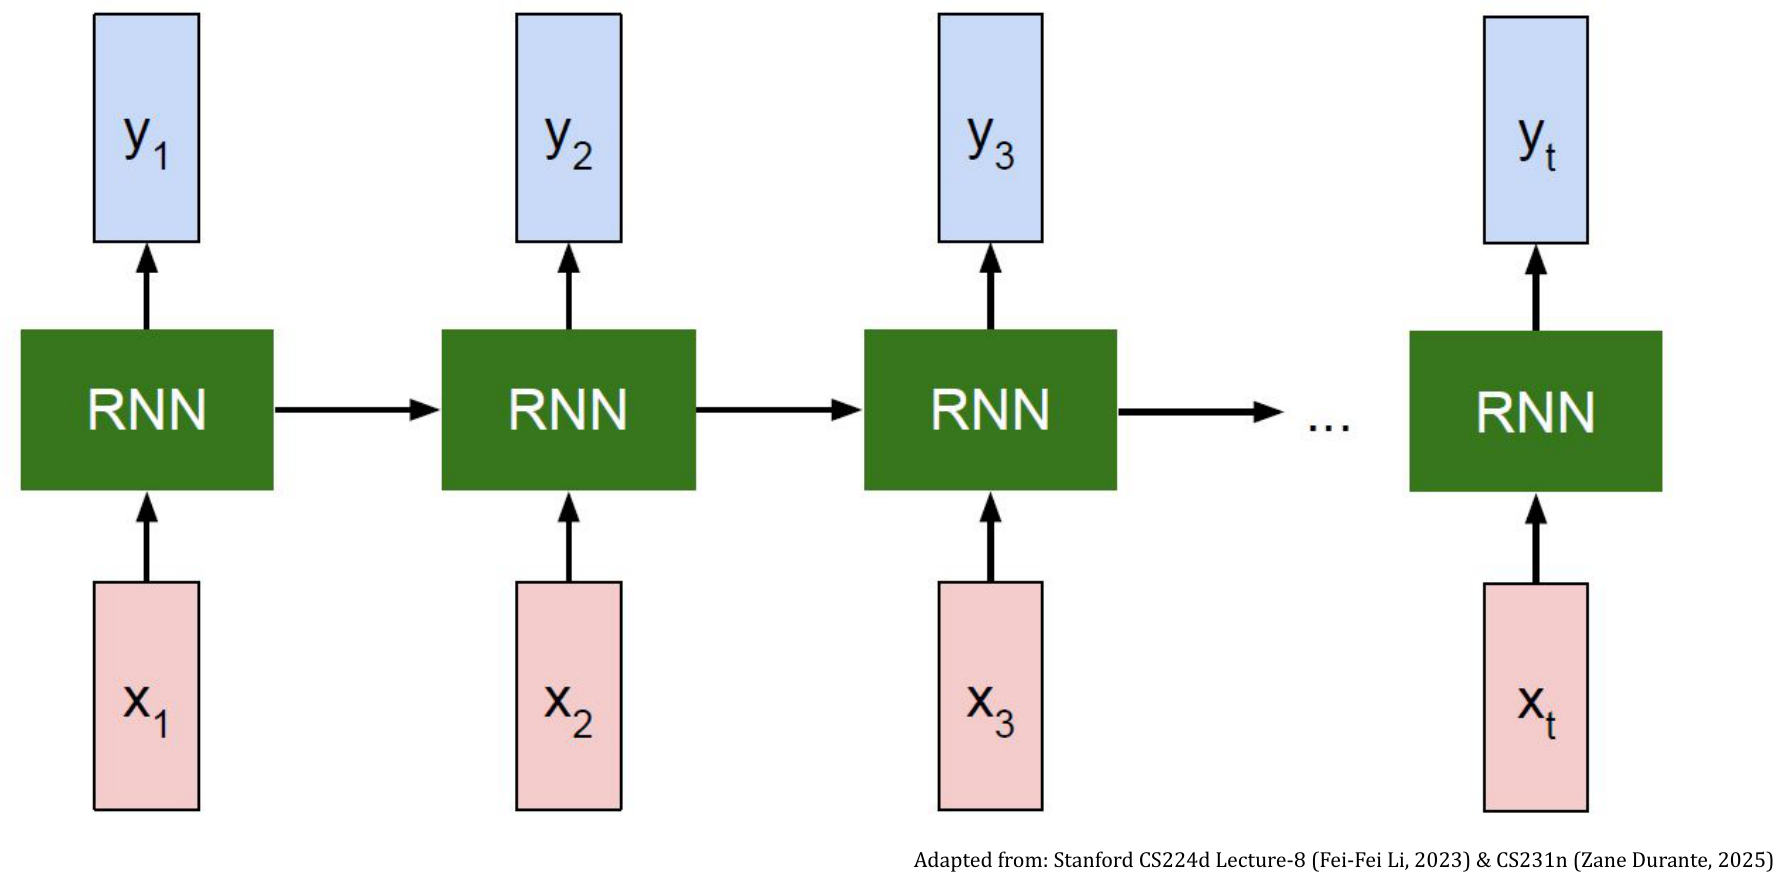
\includegraphics[width=\linewidth,height=0.95\paperheight,keepaspectratio]{images/rnn-lstm-gru/rnn_unrolled_cells_sequence.png}
\end{frame}

\begin{frame}{}
  \LARGE RNN : \textbf{Mathematical Formulations}
\end{frame}

\begin{frame}{Math in Simple RNNs}
  \begin{itemize}
  \item How RNNs propagate information (Through time!)
  \item How RNNs make predictions
  \end{itemize}
\end{frame}

\begin{frame}{A Vanilla RNN}
  \begin{figure}
    \centering
    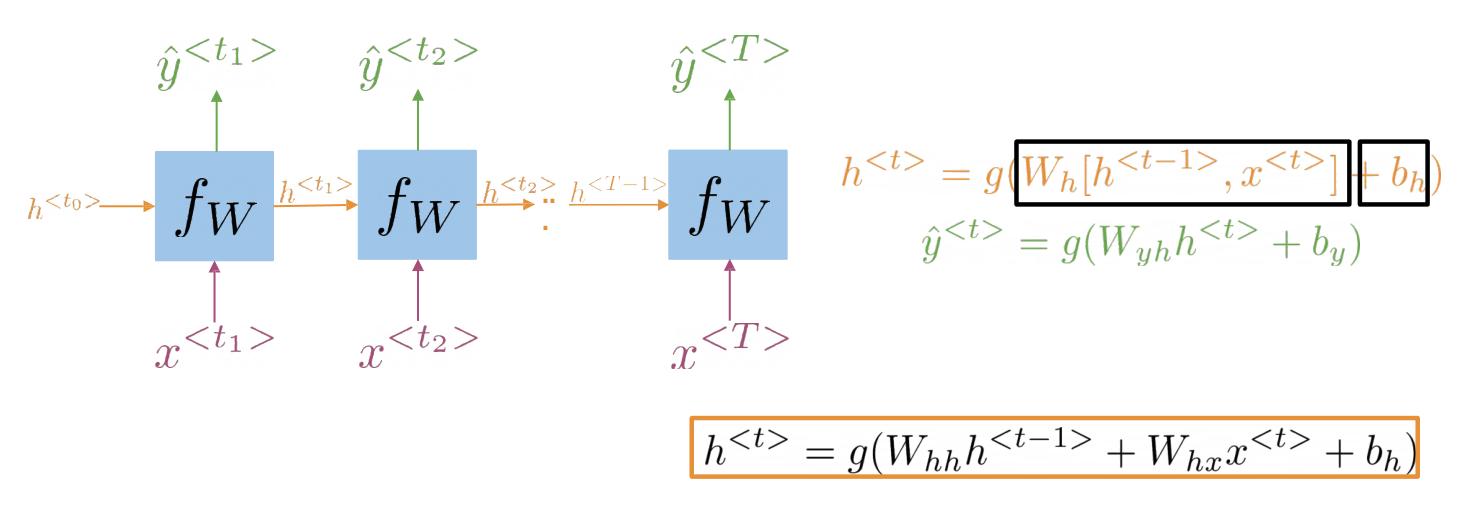
\includegraphics[width=\linewidth,height=0.66\paperheight,keepaspectratio]{images/rnn-lstm-gru/rnn_forward_pass_equations.png}
    \caption*{\tiny Source: DeepLearning.AI NLP Specialization, Course 3: Natural Language Processing with Sequence Models, Week 2 (Y. Bensouda Mourri \& L. Kaiser)}
  \end{figure}
\end{frame}

\begin{frame}{A Vanilla RNN}
  \begin{figure}
    \centering
    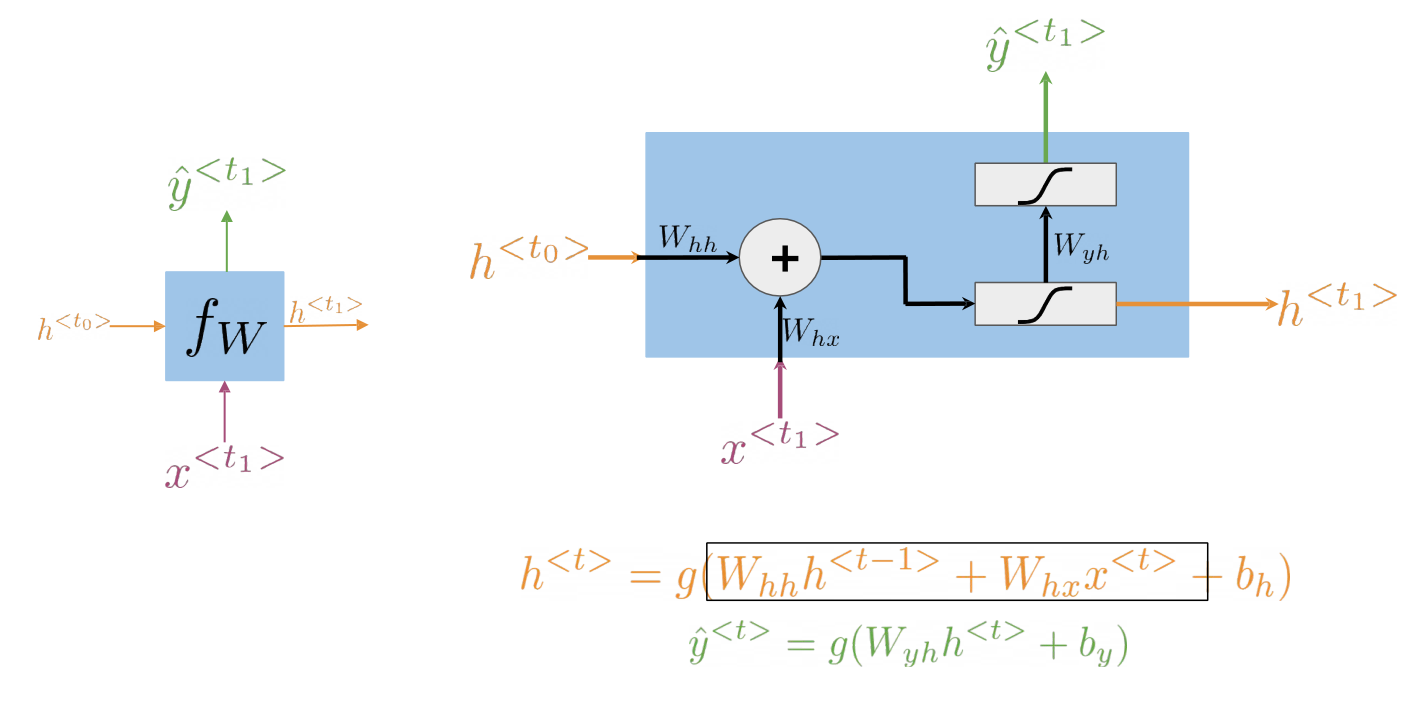
\includegraphics[width=0.9\paperwidth,height=0.66\paperheight,keepaspectratio]{images/rnn-lstm-gru/rnn_cell_internal_computation.png}
    \caption*{\tiny Source: DeepLearning.AI NLP Specialization, Course 3: Natural Language Processing with Sequence Models, Week 2 (Y. Bensouda Mourri \& L. Kaiser)}
  \end{figure}
\end{frame}

\begin{frame}{A Vanilla RNN}
  \begin{columns}[c]
    \column{0.4\textwidth}
      \centering
      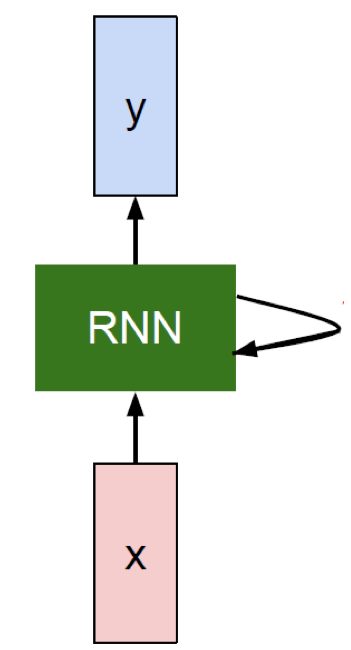
\includegraphics[width=\textwidth,height=0.8\textheight,keepaspectratio]{images/rnn-lstm-gru/rnn_single_cell_recurrence.png}
    \column{0.6\textwidth}
      \small
      \textbf{The state consists of a single ``hidden'' vector $\mathbf{h}$:}
      \vspace{0.5em}
      \begin{align*}
        \mathbf{h}_t &= f_W(\mathbf{h}_{t-1}, \mathbf{x}_t)
        \\
        \mathbf{h}_t &= \tanh(W_{hh}\mathbf{h}_{t-1} + W_{xh}\mathbf{x}_t)
        \\
        \mathbf{y}_t &= W_{hy} \mathbf{h}_t
      \end{align*}
      \vspace{0.5em}
      \begin{itemize}
        \item Sometimes called a ``Vanilla RNN'' or an \emph{Elman RNN} after Prof. Jeffrey Elman.
      \end{itemize}
      {\scriptsize
      \textit{Adapted from: Stanford CS231n (2022), Lecture 10: Recurrent Neural Networks.}
      }
  \end{columns}
\end{frame}

\begin{frame}{}
  \LARGE RNN : \textbf{Parameter Sharing}
\end{frame}

\begin{frame}{RNN: Computation Graph}
  \begin{figure}
    \centering
    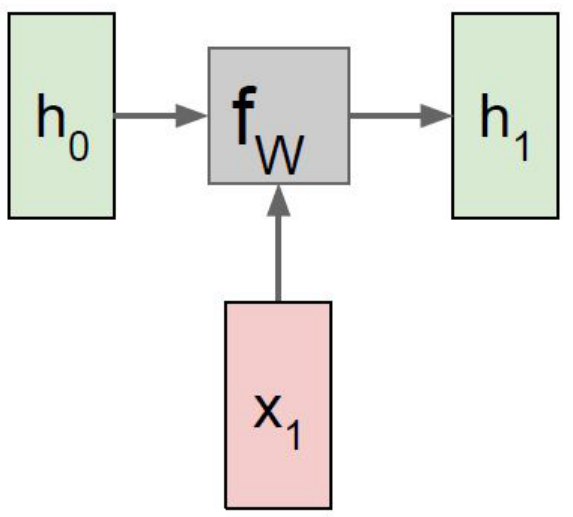
\includegraphics[width=0.9\paperwidth,height=0.66\paperheight,keepaspectratio]{images/rnn-lstm-gru/rnn_computational_graph_step1.png}
    \caption*{\tiny Source: Stanford CS231n (2022), Lecture 10: Recurrent Neural Networks}
  \end{figure}
\end{frame}

\begin{frame}{RNN: Computation Graph}
  \begin{figure}
    \centering
    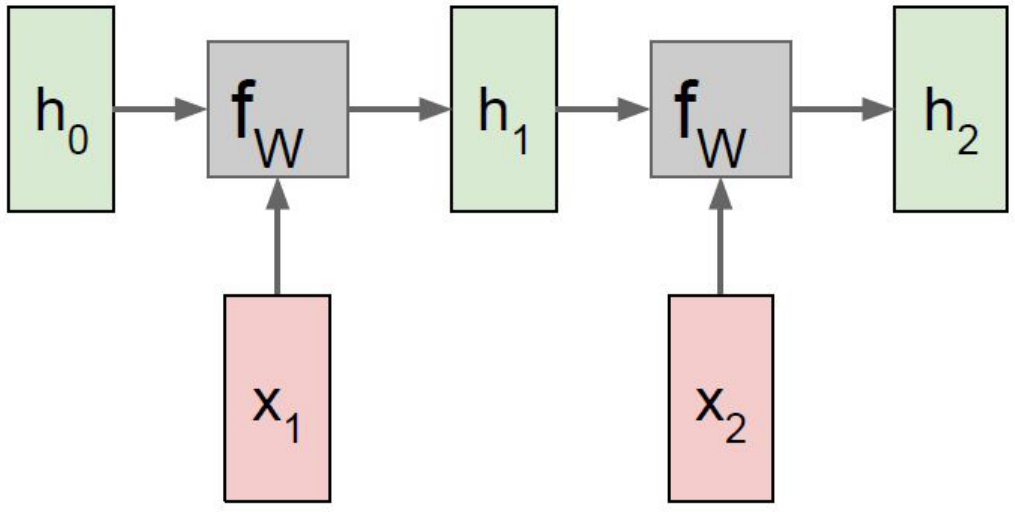
\includegraphics[width=0.9\paperwidth,height=0.66\paperheight,keepaspectratio]{images/rnn-lstm-gru/rnn_computational_graph_step2.png}
    \caption*{\tiny Source: Stanford CS231n (2022), Lecture 10: Recurrent Neural Networks}
  \end{figure}
\end{frame}

\begin{frame}{RNN: Computation Graph}
  \begin{figure}
    \centering
    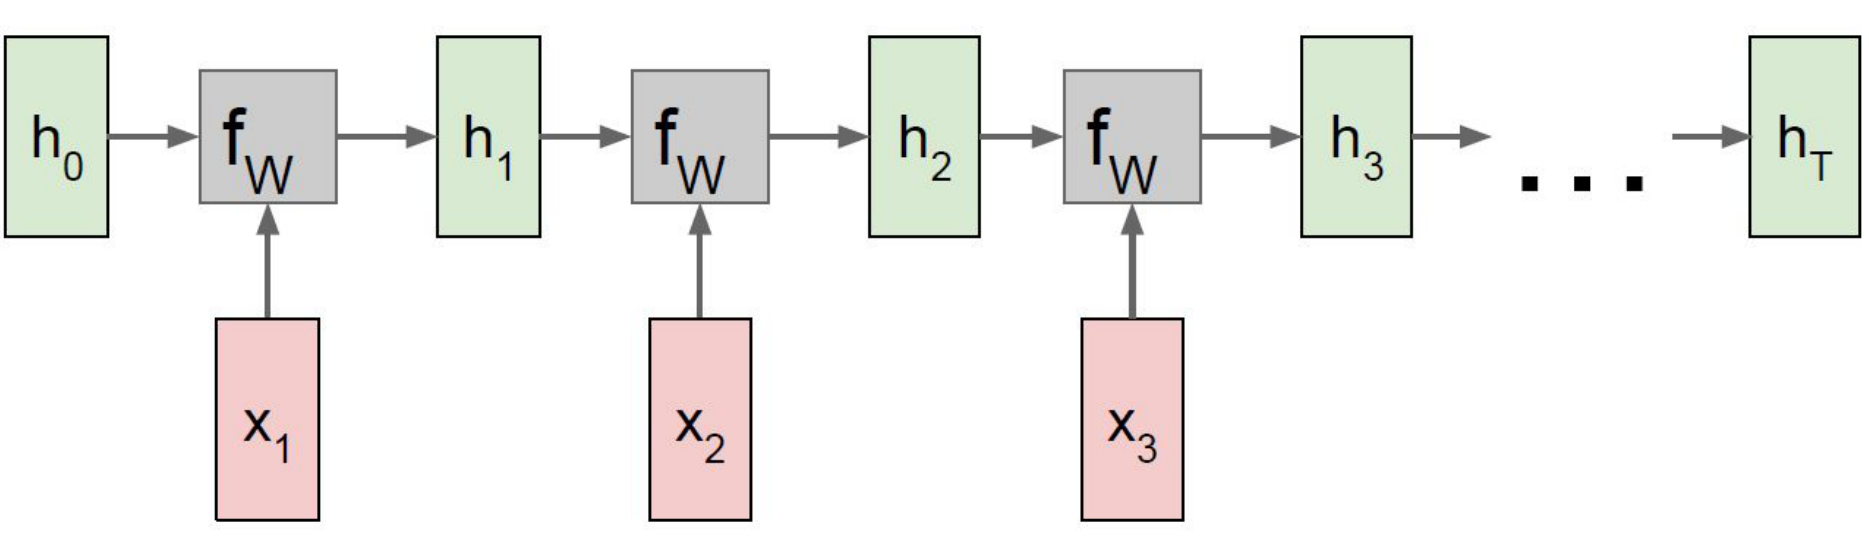
\includegraphics[width=\linewidth,height=0.66\paperheight,keepaspectratio]{images/rnn-lstm-gru/rnn_computational_graph_unrolled.png}
    \caption*{\tiny Source: Stanford CS231n (2022), Lecture 10: Recurrent Neural Networks}
  \end{figure}
\end{frame}

\begin{frame}{RNN: Computation Graph}
  \begin{figure}
    \centering
    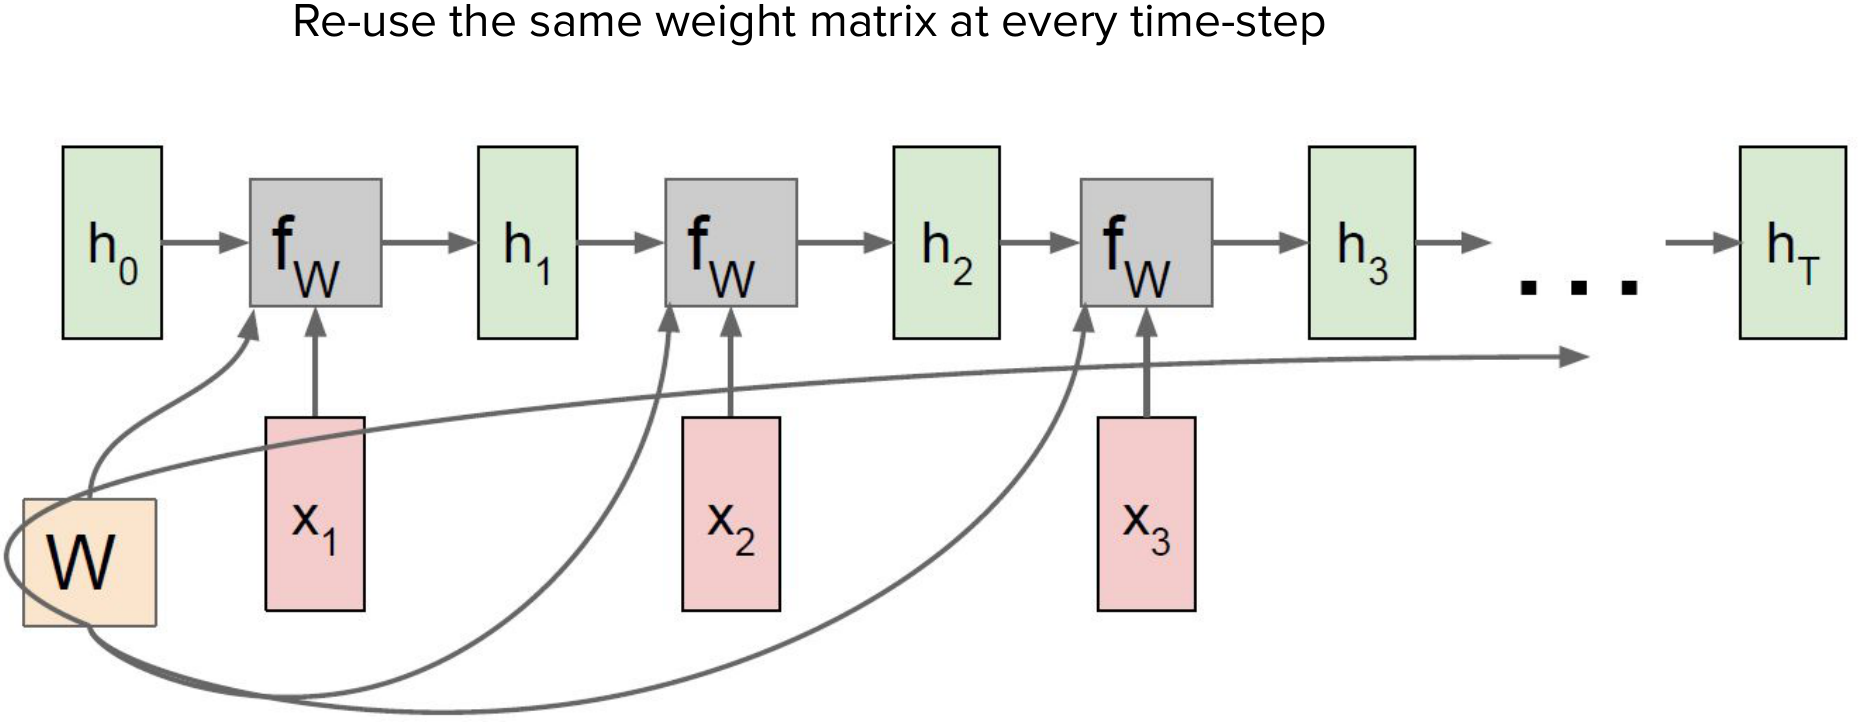
\includegraphics[width=\linewidth,height=0.66\paperheight,keepaspectratio]{images/rnn-lstm-gru/rnn_shared_weights_hidden.png}
    \caption*{\tiny Source: Stanford CS231n (2022), Lecture 10: Recurrent Neural Networks}
  \end{figure}
\end{frame}

\begin{frame}{RNN Computation Graph - Many to Many}
  \begin{figure}
    \centering
    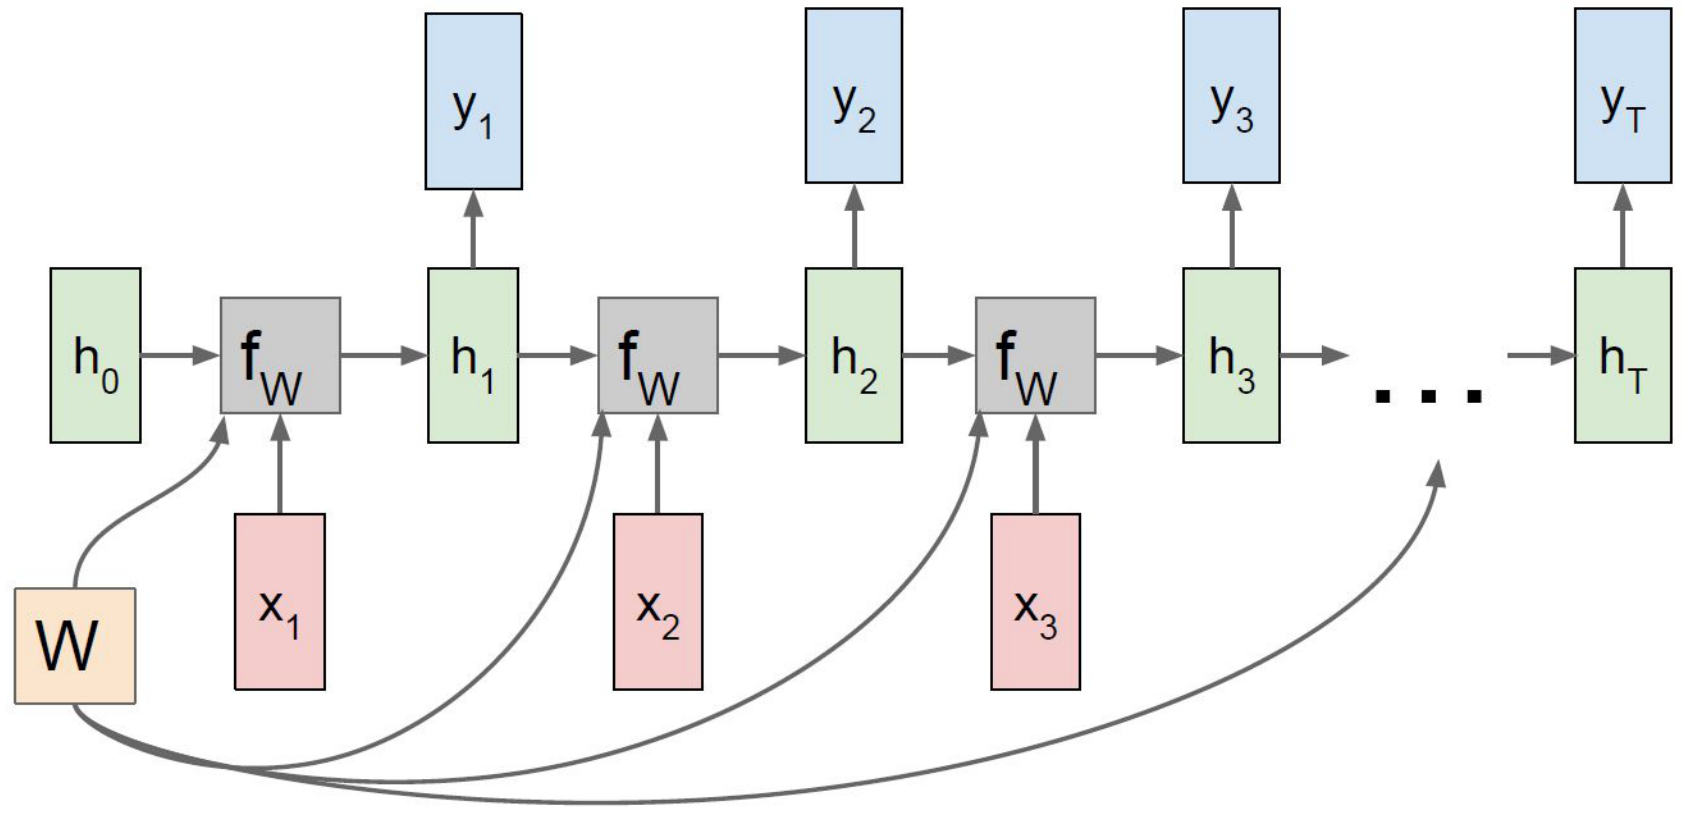
\includegraphics[width=0.9\paperwidth,height=0.66\paperheight,keepaspectratio]{images/rnn-lstm-gru/rnn_shared_weights_with_outputs.png}
    \caption*{\tiny Source: Stanford CS231n (2022), Lecture 10: Recurrent Neural Networks}
  \end{figure}
\end{frame}

\begin{frame}{RNN Computation Graph - Many to Many}
  \begin{figure}
    \centering
    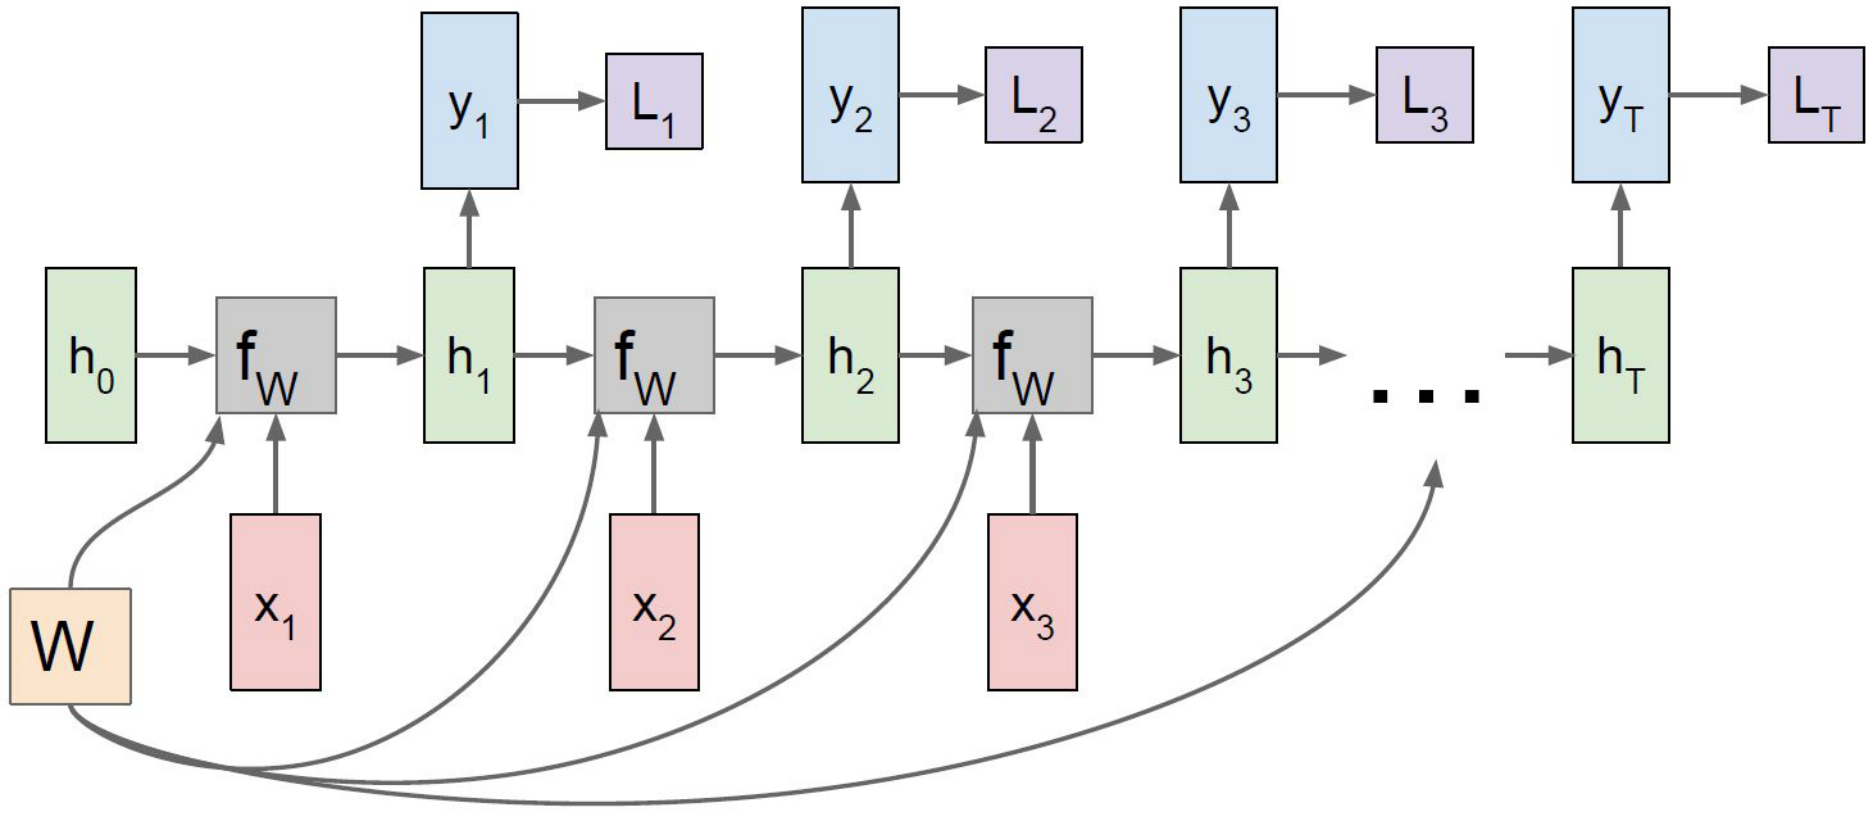
\includegraphics[width=0.9\paperwidth,height=0.66\paperheight,keepaspectratio]{images/rnn-lstm-gru/rnn_per_timestep_loss.png}
    \caption*{\tiny Source: Stanford CS231n (2022), Lecture 10: Recurrent Neural Networks}
  \end{figure}
\end{frame}

\begin{frame}{RNN Computation Graph - Many to Many}
  \begin{figure}
    \centering
    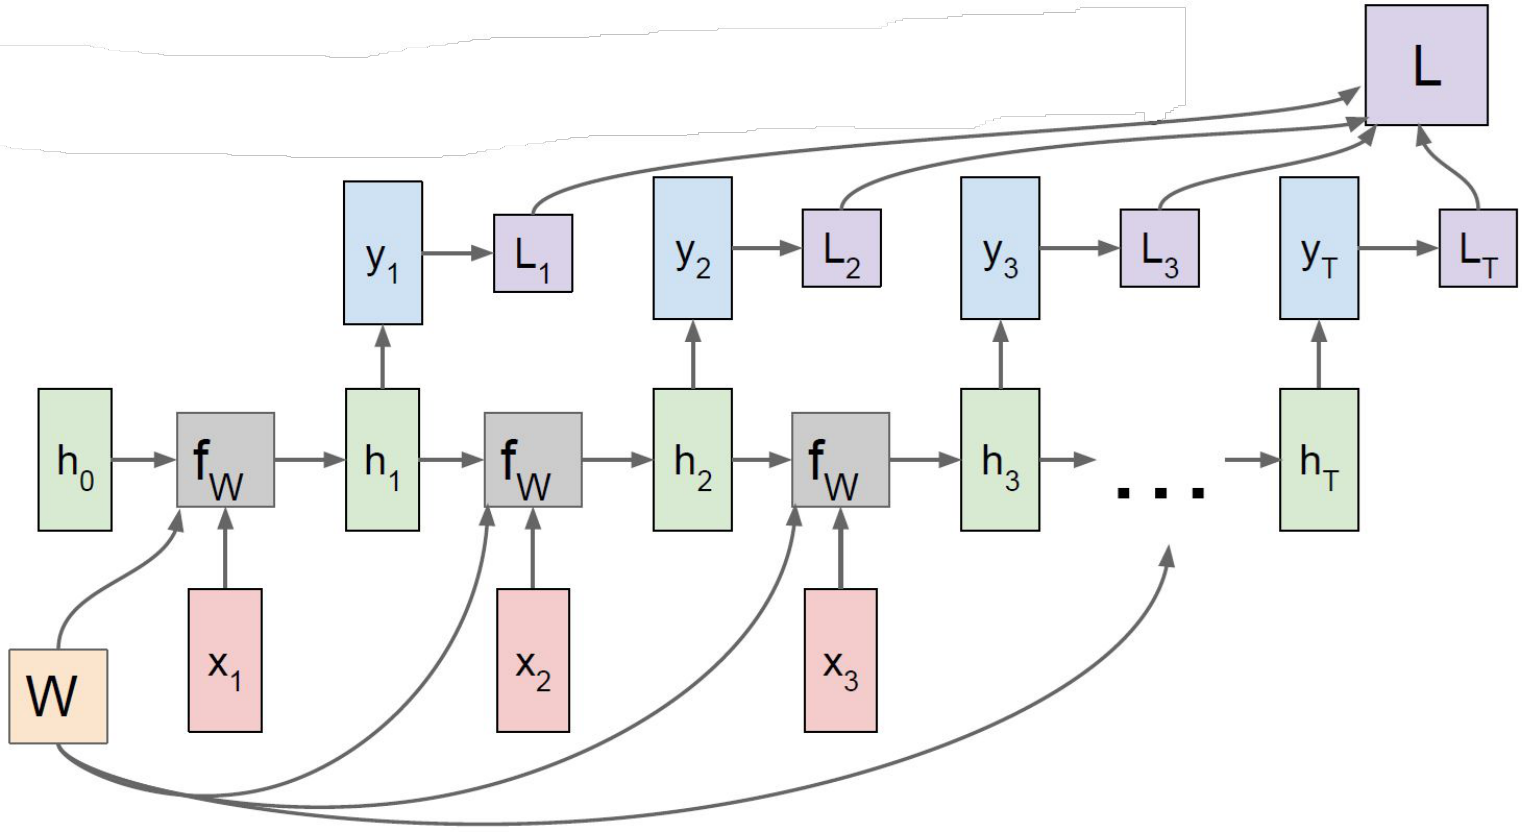
\includegraphics[width=0.9\paperwidth,height=0.66\paperheight,keepaspectratio]{images/rnn-lstm-gru/rnn_total_loss_aggregation.png}
    \caption*{\tiny Source: Stanford CS231n (2022), Lecture 10: Recurrent Neural Networks}
  \end{figure}
\end{frame}
